\section{Einführung}


Seit einigen Jahren entscheiden sich immer mehr Menschen Urlaub auf einem Campingplatz zu machen 
\cite{periodical:ANST}. Der Gedanke an Menschenmassen und Fallen für Touristen schreckt die Leute von 
den typischen Touristenzielen ab. Zudem ist der Kontakt zu der Natur für viele ein wichtiger Teil 
in einem Urlaub. In den letzten anderthalb Jahren stieg die Anzahl von Campinplatzbesuchern rasant
\cite{periodical:UBST}. Die Corona-Pandemie drängte die Leute dazu, Urlaubsmöglichkeiten zu suchen, 
bei denen das Risiko von einer Infektion niedrig sei und wo genug Abstand gehalten werden könne
\cite{periodical:AUST}. Da viele Hotels und andere Ferieneinrichtungen geschlossen waren, blieb 
vielen Leuten, besonders Familien, nichts anderes übrig, als die Ferien etwas anders zu organisieren 
und gestalten 

\vfill
\begin{figure}[H]
    \centering{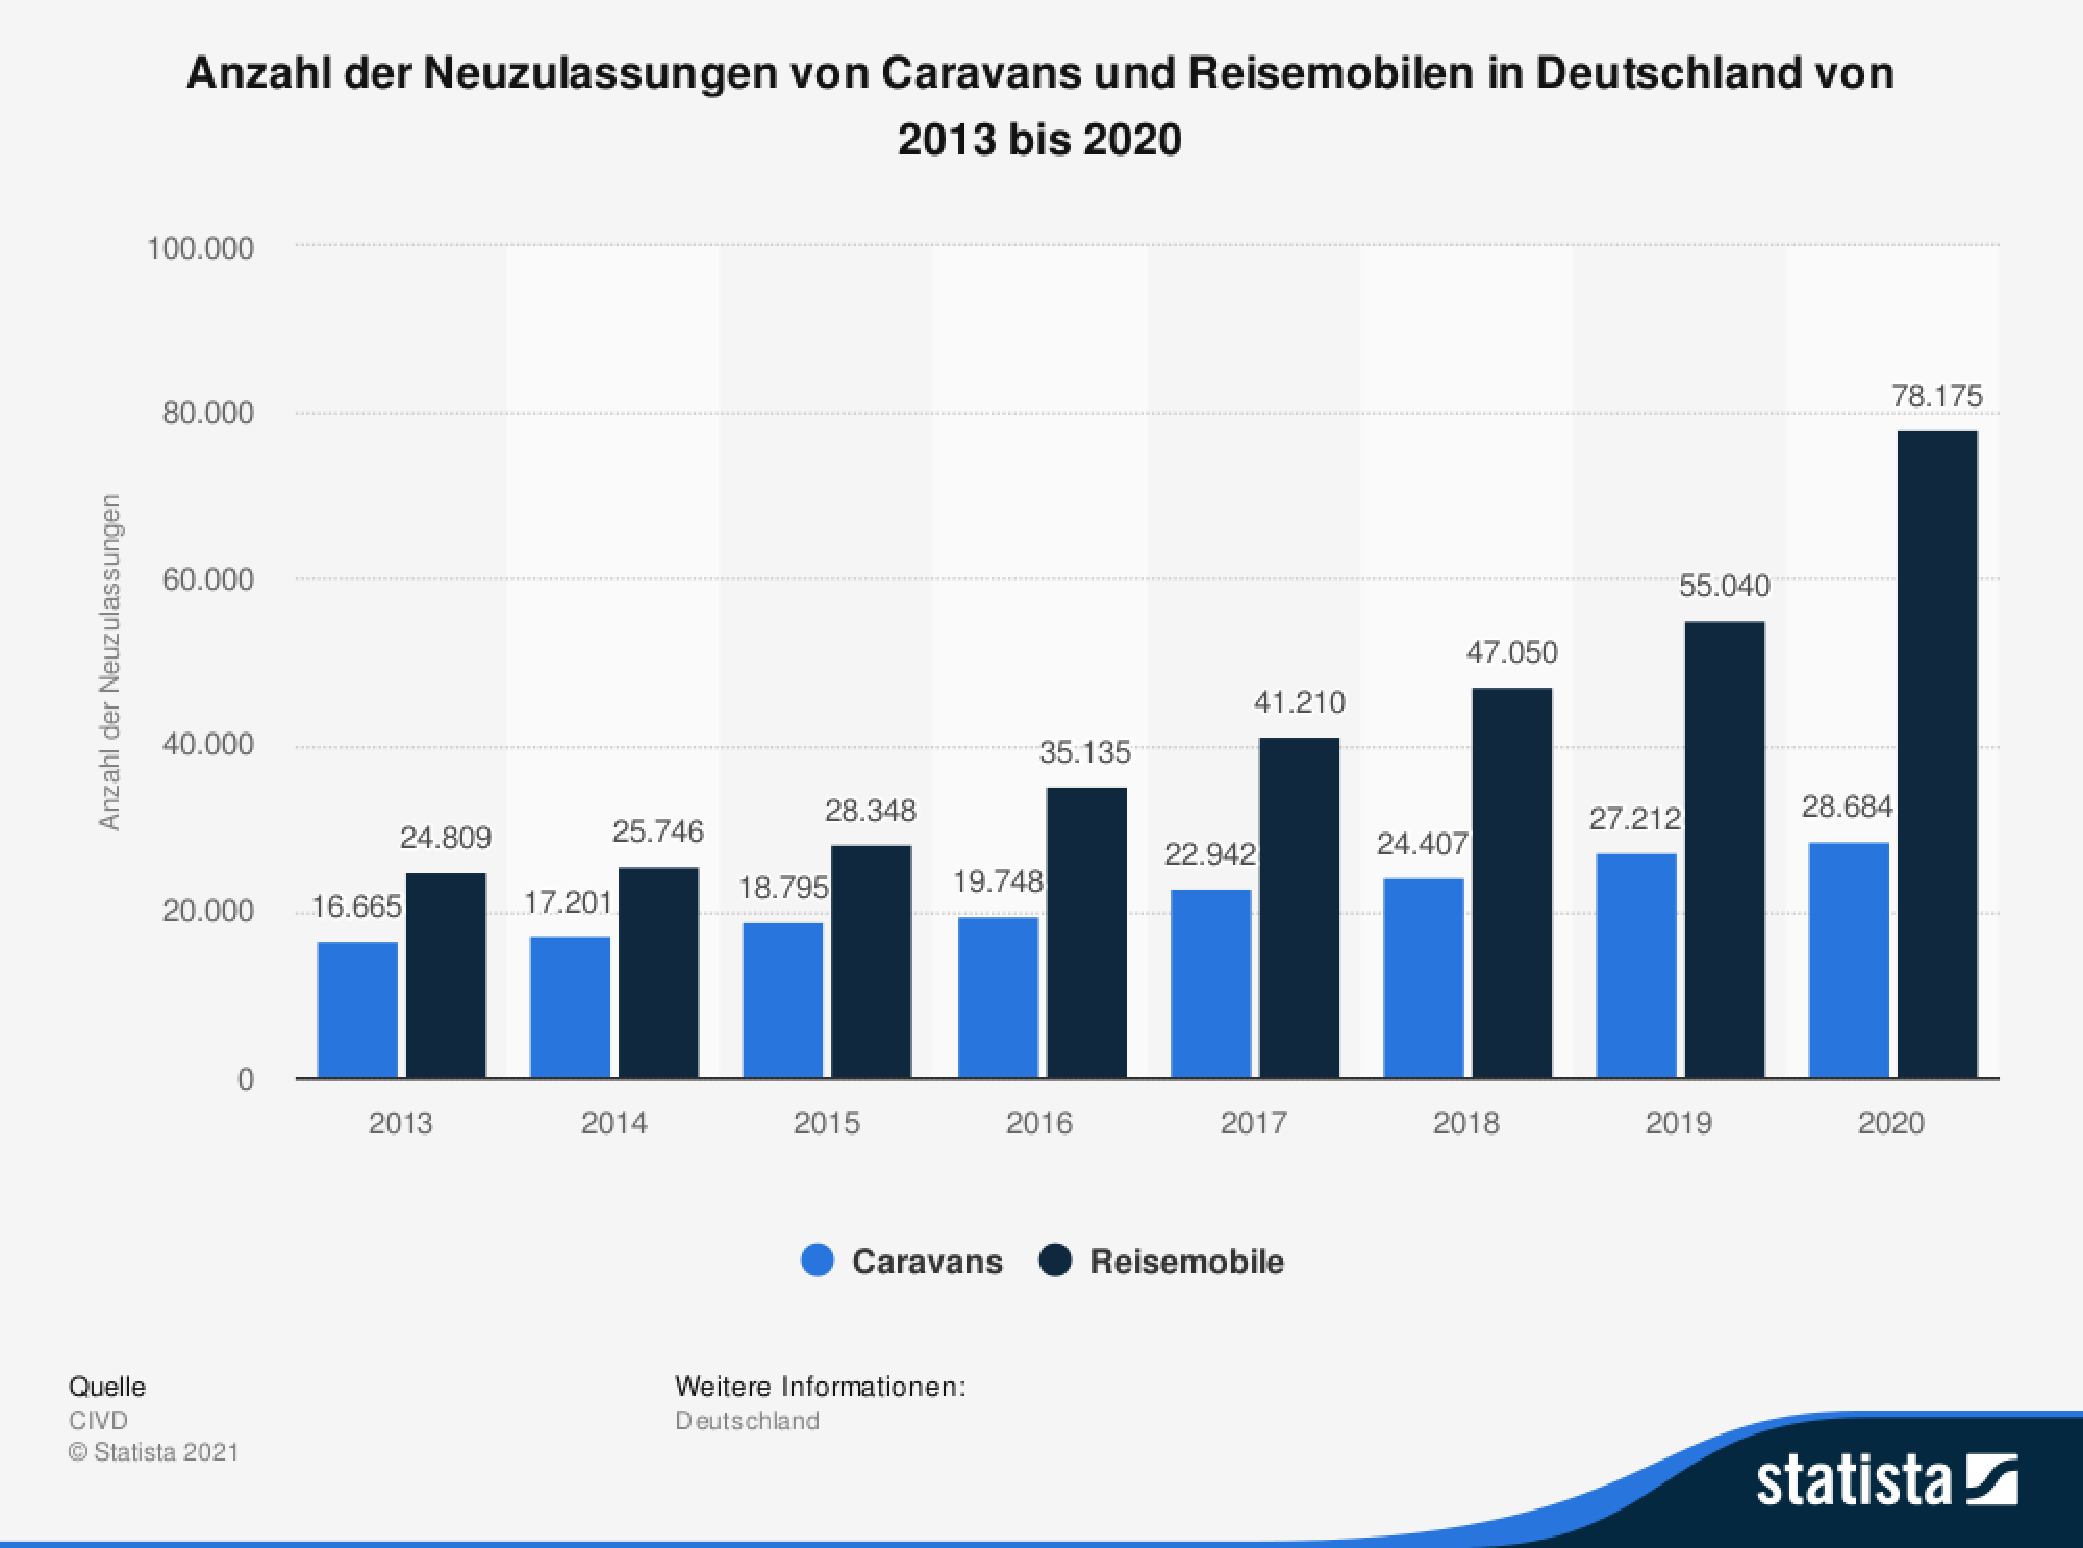
\includegraphics[width=12cm]{Bilder/periodical_ANST}}
    \caption{Neuzulassungen von Caravans und Reisemobilen (2013-2020) \\ Quelle: \cite{periodical:UBST}}
    \label{fig:periodical_ANST}
\end{figure}
%\vfill

Die traditionelle Idee von Campingplätzen, bei der Jugendliche oder Familien weit entfernt von der 
Gesellschaft sind, ist heute eine andere. Heute wollen Urlauber auf den Kontakt mit der Natur
möglichst nicht verzichten, wodurch Campingplätze immer voller werden. Aus diesem Grund wäre es
sinnvoll, die Möglichkeiten zur Grundversorgung zu erweitern, ohne direkt einen neuen Supermarkt
bauen zu müssen. In dieser Hinsicht kann die Einrichtung eines elektronischen Click-and-Buy-Automaten
\footnote{Die Waren werden online bezahlt und zu einem gewünschten Zeitpunkt können sie angeholt
werden \cite{refart:ECPG}.}, der mit einem Automaten zu vergleichen ist, eine wesentliche Rolle 
spielen, um einen Campingplatz und die Gegend drum herum zu modernisieren, die Möglichkleiten 
zur Grundversorgung zu erweitern und ihn attraktiver für Reisende und die Leute auf dem Land zu machen.


Da die Errichtung eines solch Automaten aus verschiedene Bestandteilen besteht, wie die Verkabelung 
für den Netzwerkzugang, der physischer Aufbau für den Automat und die Software für den Kundenzugang, 
konzentrieren wir uns hier auf mögliche Zahlungsverfahren für unseren Automaten. Die Sicherheit der 
digitalen Zahlungsmethoden stellt eine der wichtigsten Herausforderung für die Entwicklung eines 
solchen Systems dar. Vernachlässigungen in diesem Bereich führen auf der einen Seite zu unberechenbarem
Vertrauensverlust seitens der potenziellen Nutzenden und auf der anderen Seite zu finanziellen und 
moralischen Schäden der direkten Stakeholder. Die geplante Wissenschaftliche Arbeit soll folgende 
Frage behandeln: Wie kann sicheres bargeldloses Bezahlen in einem Click-and-Buy-Automat gewährleistet
werden? 

\vspace*{1cm}
\begin{figure}[H]
    \centering{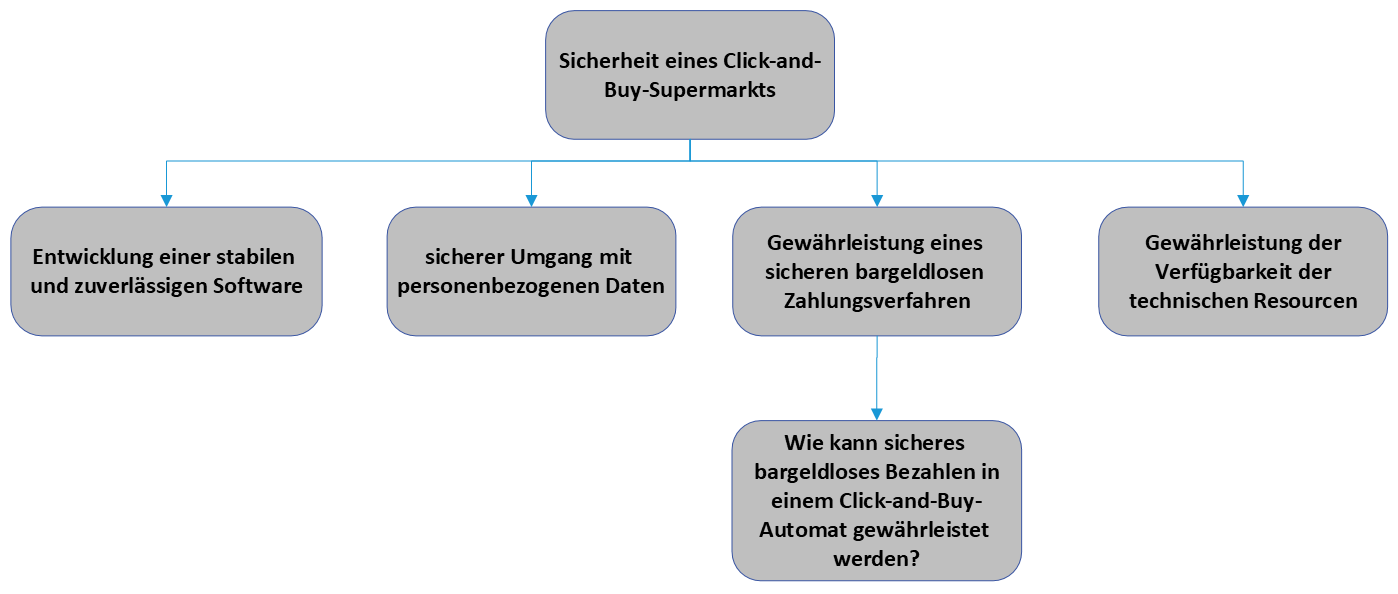
\includegraphics[width=15cm]{Bilder/Diagram_Einfuehrung.png}}
    \caption{Forschungsfrage \\ Quelle: eigene Darstellung}
    \label{fig:diagramrecherche}
\end{figure}